%%%%%%%%%%%%%%%%%%%%%%%%%%%%%%%%%%%%%%%%%%%%%%%%%%%%%%%%%%%%%%%%%%%%%%%%%%%%%%%%
\documentclass[twocolumn]{revtex4}

%%%%%%%%%%%%%%%%%%%%%%%%%%%%%%%%%%%%%%%%%%%%%%%%%%%%%%%%%%%%%%%%%%%%%%%%%%%%%%%%
% Note that comments begin with a "%" and are not turned into text in the .pdf
% document.
%%%%%%%%%%%%%%%%%%%%%%%%%%%%%%%%%%%%%%%%%%%%%%%%%%%%%%%%%%%%%%%%%%%%%%%%%%%%%%%%

%%%%%%%%%%%%%%%%%%%%%%%%%%%%%%%%%%%%%%%%%%%%%%%%%%%%%%%%%%%%%%%%%%%%%%%%%%%%%%%%
% Include some extra packages.
%%%%%%%%%%%%%%%%%%%%%%%%%%%%%%%%%%%%%%%%%%%%%%%%%%%%%%%%%%%%%%%%%%%%%%%%%%%%%%%%
\usepackage[]{graphicx}
%%%%%%%%%%%%%%%%%%%%%%%%%%%%%%%%%%%%%%%%%%%%%%%%%%%%%%%%%%%%%%%%%%%%%%%%%%%%%%%%

%%%%%%%%%%%%%%%%%%%%%%%%%%%%%%%%%%%%%%%%%%%%%%%%%%%%%%%%%%%%%%%%%%%%%%%%%%%%%%%%
\begin{document}

%%%%%%%%%%%%%%%%%%%%%%%%%%%%%%%%%%%%%%%%%%%%%%%%%%%%%%%%%%%%%%%%%%%%%%%%%%%%%%%%
\title{
Journal article
}

\author{T.~King}
\affiliation{Siena College, Loudonville, NY}

\date{12/14/2015}

\begin{abstract}
	This project is about determining whether or not a Velociraptor can catch up to a person and then bite them. I made a graph to show the position over time of the person and the raptor and then added an arrow to show where the raptor is when it is only one meter behind the person. I then calculated the probability    
of the raptor biting the person when it is a meter behind them. It is more than likely that a person will get away from a raptor if they have a 30 meter head start. The analysis shows that I understand what each question is asking.    
\end{abstract}

\maketitle
%%%%%%%%%%%%%%%%%%%%%%%%%%%%%%%%%%%%%%%%%%%%%%%%%%%%%%%%%%%%%%%%%%%%%%%%%%%%%%%%

%%%%%%%%%%%%%%%%%%%%%%%%%%%%%%%%%%%%%%%%%%%%%%%%%%%%%%%%%%%%%%%%%%%%%%%%%%%%%%%%
\section{Graphs}
%%%%%%%%%%%%%%%%%%%%%%%%%%%%%%%%%%%%%%%%%%%%%%%%%%%%%%%%%%%%%%%%%%%%%%%%%%%%%%%%
This graph is showing the position versus time of the human running at 3 $m/s$ and the velociraptor running at 18 $m/s$. The raptor catches up to the person at after 2 seconds. The person has a 30$m$ head start also.

\begin{figure}[h]	
	\centering
	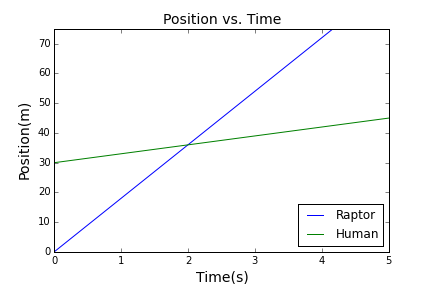
\includegraphics[width=0.5\textwidth]{PvT.png}
	\caption{This shows position versus time \label{fig:graph}}	
\end{figure}

%%%%%%%%%%%%%%%%%%%%%%%%%%%%%%%%%%%%%%%%%%%%%%%%%%%%%%%%%%%%%%%%%%%%%%%%%%%%%%%%
\section{Algebra}
To find out the when the human and raptor collide I used:
$$p = 3 * x + 30$$
and
$$r = 18 * x$$
This shows that the person has a 30 meter head start and is running at 3 meters per seconds. The raptor is starting at 0 and runs at 18 meters per second.
$$X_r_i = 0$$

$$V_r_i = 18 m/s$$

$$X_h_i = 30 m$$

$$V_h_i = 3 m$$

$$a = 0 m/s^2$$

$$X_r_f = X_r_i + V_r_i(t) + 0.5(a)(t)^2$$

$$X_r_f = V_r_i(t)$$

$$X_h_f = X_h_i + V_h_i(t) + 0.5(a)(t)^2$$

$$X_h_f = X_h_i + V_h_i(t)$$

$$X_r_f = X_h_f$$

$$V_r_i(t) = X_h_i + V_h_i(t)$$

$$V_r_i(t) - V_h_i(t) = X_h_i$$

$$t(V_r_i - V_h_i) = X_h_i$$

$$t = X_h_i/(V_r_i - V_h_i)$$

$$t = 30/(18-3)$$

$$t = 2(s)$$

To find out when the raptor is one meter behind the person:
I used $p = (3* x + 30)$ and $r = (18 * x)$. The p is for person and r is for raptor. When those to values are equal it will tell me what the x is in seconds.
Given:

$$t = 2(s)$$

$$X_H_f = X_H_i + V_H_i(t) + .5(a)(t^2)$$
$$X_H_f = X_H_i + V_H_i(t)$$
$$X_H_f = 30 + (3(2))$$
$$X_H_f = 36 (m)$$

$$X_R_f = 35 (m)$$ 

$$X_R_f = X_R_i + V_R_i(t) + .5(a)(t^2)$$	
$$X_R_f = V_R_i(t)$$ 
$$t = X_F_i / V_R_i$$
$$t = 35 / 18$$
$$t = 1.94 (s)$$
%%%%%%%%%%%%%%%%%%%%%%%%%%%%%%%%%%%%%%%%%%%%%%%%%%%%%%%%%%%%%%%%%%%%%%%%%%%%%%%%
\section{Will it bite you?}
I generated a 3 different numbers between 0 and 100 to try and find out if they raptor will bite the person. If the first number is less than 20 then the raptor bite the person. If not then they got away and the raptor will try again. If they second number is less than 15 then the person was bitten. If the raptor misses the seconds time it will try again and the person will get away if the third number is above 7. The raptor has to miss all three times for the person to get away. Every time the person gets away it will add 1 to the variable i set as success. To find the probability of escape I used the equation $(success/float(1000))*100$. It generates 1000 numbers for each time the raptor tries to bite. This equation will show how likely the person is to get away from the raptor. The person usually gets away about 60 percent of the time.
%%%%%%%%%%%%%%%%%%%%%%%%%%%%%%%%%%%%%%%%%%%%%%%%%%%%%%%%%%%%%%%%%%%%%%%%%%%%%%%%
\end{document}
%%%%%%%%%%%%%%%%%%%%%%%%%%%%%%%%%%%%%%%%%%%%%%%%%%%%%%%%%%%%%%%%%%%%%%%%%%%%%%%%
